\documentclass{article}

\usepackage[UTF8]{ctex}
\usepackage[
  a4paper,
  left=2.5cm,
  right=2.5cm,
  top=2.5cm,
  bottom=2.5cm,
  headsep=0.5cm,
  footskip=1cm
]{geometry}
\usepackage{titling}
\usepackage{amsmath}
\usepackage{amsfonts}
\usepackage{amssymb}
\usepackage{amsthm}
\usepackage{minted}
\usepackage{graphicx}
\usepackage{booktabs}

\renewcommand{\maketitlehookb}{
  \ifx\theauthor\empty
  \vspace{-3em}
  \else
  \begin{center}
    \textbf{\theauthor}
  \end{center}
  \fi
}

\title{分布式能源配电网风险分析}
\author{}
\date{\today}

\begin{document}
\maketitle

\begin{abstract}\label{sec:abstract}
  摘要

  \textbf{关键词:} 关键词1,关键词2,关键词3
\end{abstract}

\newpage

\section{问题重述}\label{sec:problem}

\subsection{问题背景}\label{sec:background}

随着全球能源转型和我国"双碳"目标的深入推进,可再生分布式能源(如光伏、风电)在配电网中的渗透率显著提升。
这种趋势不仅推动了清洁能源的利用,还对传统配电网的运行方式提出了新的挑战。
传统配电网设计以集中式发电和单向潮流为主,难以适应分布式能源出力波动性和不确定性带来的复杂运行场景。
分布式能源的接入改变了配电网的潮流分布,可能导致失负荷(因故障导致供电中断)或过负荷(线路电流超额定载流量10\%以上),从而增加系统运行风险。
此外,联经开关的存在为故障后功率转移提供了可能,但其操作复杂性进一步增加了风险评估的难度。
在实际应用中,不同类型用户(如工业、商业、政府机构)对供电中断的敏感度差异显著,需综合考虑经济损失和社会影响来量化风险。
现有研究多聚焦于分布式能源的接入技术或单一风险因素,缺乏对失负荷与过负荷风险的系统性建模与综合评估。
本研究基于62节点有源配电网系统,结合分布式能源的运行特性,构建风险评估模型,为配电网的规划与优化提供理论支持。
这种研究不仅在理论上丰富了配电网风险管理的知识体系,还在实践中为提升电网可靠性和经济性提供了科学指导,具有重要的现实意义。

\subsection{问题提出}\label{sec:problem_proposed}

本研究旨在通过数学建模量化分布式能源接入配电网后引发的失负荷与过负荷风险,为配电网的稳定运行提供系统化解决方案。
研究围绕以下核心任务展开:首先,需建立分布式能源接入配电网后失负荷与过负荷风险的数学模型,明确风险的概率分布及其危害程度,结合联经开关的功率转移机制优化风险计算。
然后,基于62节点有源配电网系统,应用所建模型分析分布式能源接入对系统风险的动态影响,揭示风险演变的规律。
这些任务通过理论建模、数据分析与仿真验证相结合,旨在为配电网运行提供科学的决策依据,提升其在高渗透率分布式能源场景下的可靠性和经济性。

\section{问题分析}\label{sec:analysis}

分布式能源接入配电网的风险评估涉及失负荷与过负荷的概率建模、风险演变分析、光伏容量影响评估及储能优化等多个子问题,呈现出高度的复杂性和综合性。
问题的核心在于分布式能源出力的波动性与不确定性对配电网潮流分布的深刻影响,这不仅改变了传统配电网的运行模式,还引入了新的风险来源。
失负荷风险源于故障导致的供电中断,其危害程度与用户类型和停电持续时间密切相关;过负荷风险则由线路电流超载引发,可能导致设备损坏或系统崩溃。
联经开关的存在为功率转移提供了灵活性,但其操作需考虑网络拓扑的动态变化,增加了建模难度。

\subsection{模型假设}\label{subsec:assumption}

为了简化模型分析,本文在建模过程中做出以下假设:

\begin{enumerate}
  \item 假设分布式能源出力为固定值,且不随时间变化。\label{assumption:fixed_output}
  \item 假设配电网中所有节点的负荷均为已知值,且不随时间变化。\label{assumption:fixed_load}
  \item 假设配电网的拓扑结构在分析期间保持不变,且电压恒定。\label{assumption:topology_fixed}
  \item 假设配电网中联络开关的容量足够大,能够承载所有可能的功率转移。\label{assumption:large_capacity}
  \item 假设配电系统故障发生独立,且故障率固定。\label{assumption:independent_failure}
\end{enumerate}

\subsection{符号说明}\label{subsec:notation}

\section{模型建立与求解}\label{sec:model}

\subsection{问题 1 建模与求解}\label{subsec:problem1}

\subsubsection{问题 1 求解思路}\label{subsubsec:problem1_idea}

问题 1 要求建立分布式能源接入配电网后失负荷与过负荷风险的数学模型,核心目标在于量化风险概率和危害程度,为进一步的分析奠定基础。
分布式能源的出力波动与联络开关的功率转移特性是影响风险评估的关键因素。
由于题目中指出,同一时刻同一类型只发生一个故障,因此可以独立分析电网中的各个节点,分别分析对应的风险。
首先,针对失负荷风险,需要分析故障单元的故障率,结合网络拓扑和联络开关状态计算失负荷概率和风险期望。
此外,考虑到不同用户类型的危害程度差异,还需要引入权重因子,量化危害程度。
其次,针对过负荷风险,需要分析电路中电流的分布情况,结合联络开关的功率转移特性,判断是否超过额定载流量的 10\%。
最后,综合考虑失负荷与过负荷风险,建立综合风险评估模型。

技术路线上,我们选择使用 Python 作为主要工具,利用 pandas 和 numpy 分析负荷和出力数据,结合 networkx 库进行图论分析, matplotlib 库进行可视化。
潜在挑战在于对于大规模节点计算的准确性,以及联络开关状态变化对风险评估的影响。

\subsubsection{问题 1 建模}\label{subsubsec:problem1_model}

为了量化分布式能源接入配电网后失负荷与过负荷风险,我们首先需要建立数学模型来描述系统的运行状态和风险评估指标。
模型以配电网的拓扑结构、负荷分布、分布式能源的出力以及联经开关的状态为输入,输出系统的风险值,风险计算公式题目中已经给出为:
\begin{equation}\label{eq:risk_formula}
  R_{\text{sys}} = P_{\text{LL}} \cdot C_{\text{LL}} + P_{\text{OL}} \cdot C_{\text{OL}}
\end{equation}
其中 $P_{\text{LL}}$ 和 $P_{\text{OL}}$ 分别表示失负荷和过负荷的概率,$C_{\text{LL}}$ 和 $C_{\text{OL}}$ 分别表示失负荷和过负荷的危害程度。

在模型中,由于假设 \ref{assumption:independent_failure},我们可以将不同节点的故障风险独立分析。
因此,我们选择枚举所有可能的故障单元,结合网络拓扑和联络开关转移功率,计算故障后的失负荷损失。
具体而言,我们可以针对故障单元的类型来讨论对应的风险评估。

当故障单元为负载时,我们认为失负荷只是因为变电站到负荷的线路故障导致,因此负载失负荷后可以从同网络的其他 dg 节点接收。
同时特殊考虑 dg 节点,认为它的失负荷损失为其出力功率。
权重因子的设置根据不同用户类型的敏感度进行调整,我们使用的具体数值如表 \ref{tab:weight_factor} 所示。
\begin{table}[h]
  \centering
  \begin{tabular}{|c|c|}
    \hline
    用户类型 & 权重因子 \\
    \hline
    工业用户 & 1.0 \\
    政府机构 & 0.8 \\
    商业用户 & 0.5 \\
    居民 & 0.2 \\
    \hline
  \end{tabular}
  \caption{不同用户类型的权重因子}
  \label{tab:weight_factor}
\end{table}
% TODO: 参考文献
形式化地说,假设故障单元为 $i$ ,其对应的负载功率或出力为 $P_i$ ,同网络的剩余容量为 $P_{\text{remain}}$ ,权重因子为 $w_i$ ,则失负荷损失为:
\begin{equation}\label{eq:loss_node}
  L_{\text{node},i} =
  \begin{cases}
    (P_i - P_{\text{remain}}) \cdot w_i & \text{if } i \text{ is a load} \\
    P_i^{dg} & \text{if } i \text{ is a dg node}
  \end{cases}
\end{equation}

当故障单元为线路时,需要考虑其影响到的节点以及联络开关的状态。
首先,我们将每条馈线抽象为一棵以变电站为根节点的树,树的每个节点都是一个负载。
那么,线路断开意味着这棵树被分为两棵树,其中一棵树的根节点为变电站,另一棵树的根节点为故障单元。
这种情况下,考虑联络开关的影响,若被影响的子树可以通过联络开关转移功率,由于前述假设 \ref{assumption:large_capacity} ,则可以假定相连馈线的所有多余功率都可以被转移到故障子树。
另外,还要考虑故障子树中的 dg 节点的出力。
为了简化分析,此时我们计算被影响子树的平均权重,以此作为这棵子树的权重,乘以其失负荷的功率作为此时的损失。
形式化地说,假设故障边的编号为 $i$ ,故障子树的节点集合为 $\mathcal{N}$ ,对应的负载功率的和为 $P_{\mathcal{N}}$ ,
dg 节点的出力功率的和为 $P_{\mathcal{N}}^{dg}$ ,从其他馈线转移的功率为 $P_{\text{transfer}}$ ,则失负荷损失为:
\begin{equation}\label{eq:loss_line}
  L_{\text{line},i} = \max\left(
    0,
    \frac{\sum_{k\in\mathcal{N}}w_k}{|\mathcal{N}|} \cdot
    (P_{\mathcal{N}} - P_{\text{transfer}} - P_{\mathcal{N}}^{dg})
  \right)
\end{equation}

当故障单元为开关时,为了简化处理,我们认为它不会影响到任何节点的功率转移,即:
\begin{equation}\label{eq:loss_switch}
  \forall i \in \mathcal{S},\quad L_{\text{switch},i} = 0
\end{equation}

综上所述,我们可以将失负荷风险 $P_{\text{LL}} \cdot C_{\text{LL}} $ 表示为:
\begin{equation}\label{eq:loss_total}
  P_{\text{LL}} \cdot C_{\text{LL}}
  = \sum_{i\in\mathcal{N}} R_{i} \cdot L_{\text{node},i}
  + \sum_{j\in\mathcal{L}} R_{j} \cdot L_{\text{line},j}
  + \sum_{k\in\mathcal{S}} R_{k} \cdot L_{\text{switch},k}
\end{equation}
其中 $\mathcal{N}$、$\mathcal{L}$ 和 $\mathcal{S}$ 分别表示故障单元为负载、线路和开关的集合。

对于过负荷风险,我们需要计算每条馈线的电流情况,判断是否超过额定载流量的 10\%。
这里我们假定馈线的电流为三相交流电,那么有功率与电压的关系为:
\begin{equation}\label{eq:current_formula}
  I = \frac{P}{\sqrt{3} \cdot U}
\end{equation}
其中 $I$ 为电流,$P$ 为功率,$U$ 为电压。

根据假设 \ref{assumption:fixed_output} 和 \ref{assumption:fixed_load},我们可以认为负载功率和出力功率是固定的。
又由假设 \ref{assumption:topology_fixed},所以可以认为馈线电流与馈线总净功率成线性关系,因此只需计算馈线的总净功率。

首先计算馈线 $i$ 的总净功率 $P_{\text{net},i}$:
\begin{equation}\label{eq:net_power}
  P_{\text{net},i} = \sum_{j\in\mathcal{N}_i} P_j - \sum_{k\in\mathcal{DG}_i} P_k^{\text{dg}}
\end{equation}
其中 $\mathcal{N}_i$ 和 $\mathcal{DG}_i$ 分别表示馈线 $i$ 上的负载节点和分布式发电节点集合。
当 $P_{\text{net},i} > 0$ 时,表示馈线 $i$ 上的负载大于分布式发电节点的出力,此时我们需要计算电流 $I_i$:
\begin{equation}\label{eq:current}
  I_i = \frac{P_{\text{net},i}}{\sqrt{3} \cdot U}
\end{equation}
否则,则考虑联络开关的功率转移。
假设联络开关能够转移的最大功率为 $P_{\text{transfer},i}$,则此时的电流 $I_i$ 为:
\begin{equation}\label{eq:current_transfer}
  I_i = \frac{|P_{\text{net},i}| - P_{\text{transfer},i}}{\sqrt{3} \cdot U}
\end{equation}

然而,由于实际上的负载和出力功率是有波动的,为了简化分析,我们认为实际上的电流成正态分布,期望值为 $I_i$,标准差为 $\sigma_i = 0.1 \cdot I_i$。
同时,由于电流本身即使没有过载也会导致线路老化等损失,因此我们给出一个分段线性的损失函数如下:
\begin{equation}\label{eq:loss_current}
  L_{\text{current},i} (I) =
  \begin{cases}
    0.2 \sqrt{3} U \frac{I}{I_{\text{rated} \cdot 1.1}} \cdot \bar{w_i} & \text{if } I_i < 1.1 \cdot I_{\text{rated}} \\
    2 \sqrt{3} U (I_i - 1.1 \cdot I_{\text{rated}} + 0.1) \cdot \bar{w_i} & \text{if } I_i \geq 1.1 \cdot I_{\text{rated}}
  \end{cases}
\end{equation}
其中 $I_{\text{rated}}$ 为馈线的额定电流,$\bar{w_i}$ 为馈线 $i$ 的平均权重。
从而计算期望损失:
\begin{equation}\label{eq:loss_current_expectation}
  P_{\text{OL}} \cdot C_{\text{OL}}
  = \sum_i E[L_{\text{current},i}]
  = \sum_i \int_{-\infty}^{+\infty} L_{\text{current},i}(I) \cdot N(I_i,\ 0.1 I_i) dI
\end{equation}
其中 $N(I_i,\ 0.1 I_i)$ 为正态分布函数。

综上所述,可以根据公式 \ref{eq:risk_formula},\ref{eq:loss_total} 和 \ref{eq:loss_current_expectation} 计算系统的风险值 $R_{\text{sys}}$。

\subsubsection{问题 1 求解}\label{subsubsec:problem1_solve}

基于所建立的数学模型,我们使用 Python 对题目给出的 62 节点有源配电网系统进行建模与求解。
我们首先使用 networkx 库构建配电网的拓扑结构,利用 pandas 和 numpy 库处理负荷和出力数据。
然后,针对每个节点的故障单元,计算其失负荷和过负荷风险。
最后,综合所有节点的风险值,得到系统的总风险值 $R_{\text{sys}}$。

首先有网络拓扑图如下:

\begin{figure}[htbp]
  \centering
  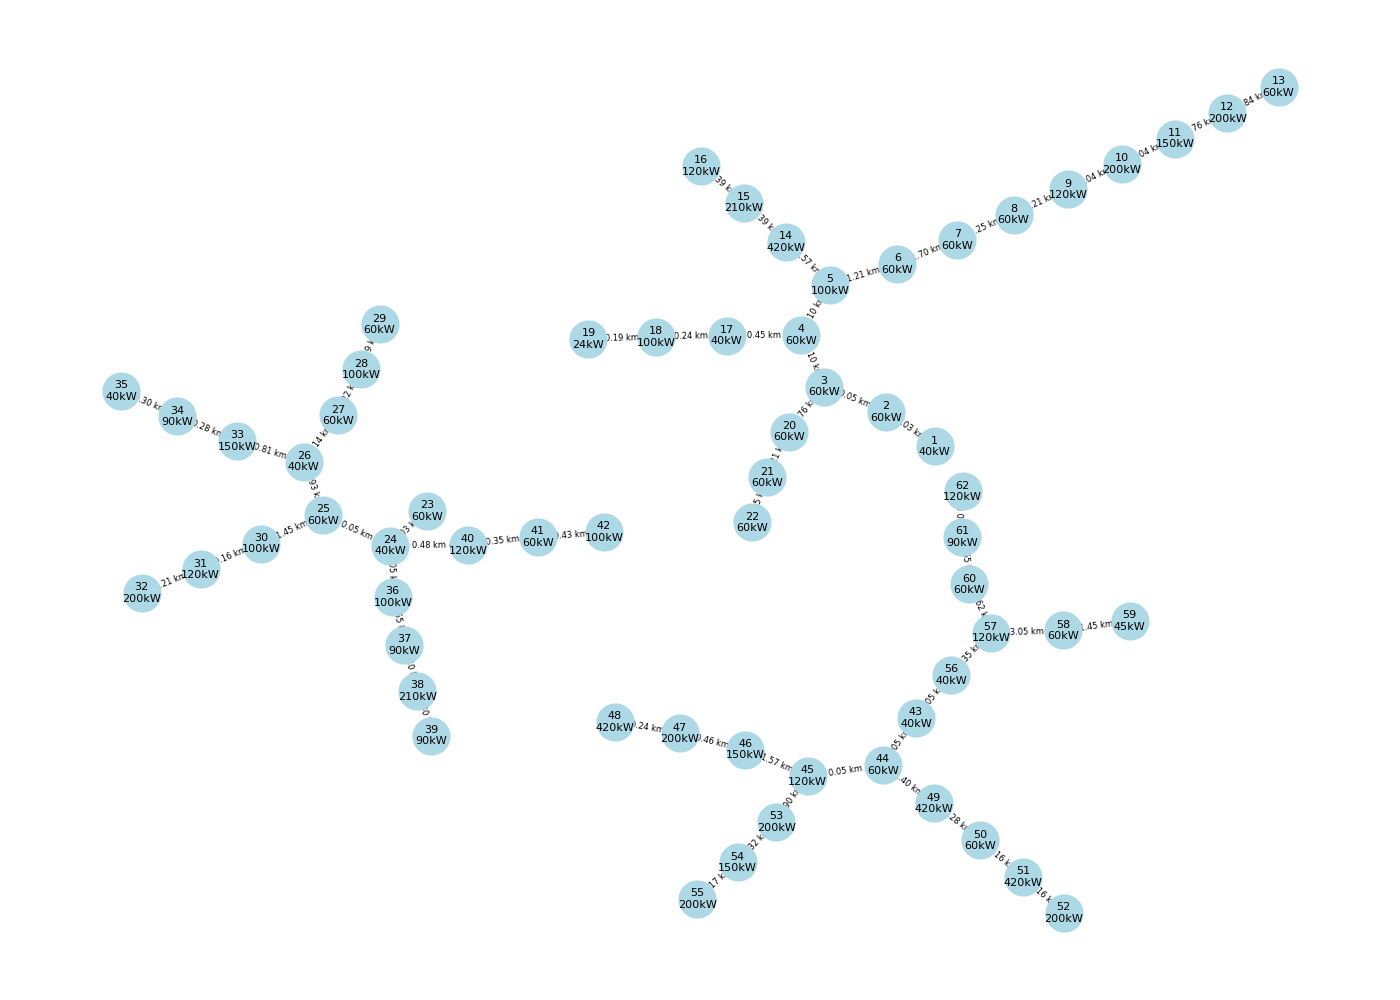
\includegraphics[width=0.8\textwidth]{problem1/topology_graph.png}
  \caption{62节点有源配电网拓扑结构}
  \label{fig:network_topology}
\end{figure}

接下来通过 Python 代码实现上述模型的求解过程,计算出系统的失负荷和过负荷风险。
分析结果表明,系统风险主要来自于失负荷风险,占总风险的 95.51\%,而过负荷风险仅占 4.49\%。
总的风险值为 36.82 ,总风险相对较高。

\subsection{问题 2 建模与求解}\label{subsec:problem2}

\subsubsection{问题 2 求解思路}\label{subsubsec:problem2_idea}

问题 2 要求分析分布式能源接入对系统风险的动态影响,揭示风险演变的规律。
核心目标是通过仿真分析分布式能源接入容量、位置等因素对系统风险的影响,量化风险演变的趋势。
我们可以通过改变分布式能源的接入容量,观察系统风险的变化。
技术路线依然使用 Python 进行仿真分析,结合 matplotlib 库进行可视化。

\subsubsection{问题 2 建模}\label{subsubsec:problem2_model}

为了衡量每个馈线承担的风险,我们为每个馈线定义风险占比。
假设整张图的边集和点集是 $\mathcal{E}$ 和 $\mathcal{N}$ ,馈线 $i$ 的边集与点集分别为 $\mathcal{E}_i$ 和 $\mathcal{N}_i$,则馈线 $i$ 的风险占比 $R_{\text{ratio},i}$ 定义为:
\begin{equation}\label{eq:ratio}
  R_{\text{ratio},i}
  = \frac
  {\sum_{j\in\mathcal{N}_i} R_j + \sum_{k\in\mathcal{E}_i} R_k}
  {\sum_{j\in\mathcal{N}} R_j + \sum_{k\in\mathcal{E}} R_k}
\end{equation}
从而可以计算出每个馈线的风险占比。

然后,我们可以通过改变分布式能源的接入容量,观察系统风险的变化。

\subsubsection{问题 2 求解}\label{subsubsec:problem2_solve}

基于所建立的数学模型,我们使用 Python 对题目给出的 62 节点有源配电网系统进行建模与求解。

首先使用 numpy 库生成分布式能源的接入容量数据,假设分布式能源的接入容量系数为 $I$ 到 $3I$ ,步长为 $0.3I$ ,其中 $I$ 为 dg 节点的出力功率。
然后,针对每个节点的故障单元,计算其失负荷和过负荷风险。
计算结果表 \ref{tab:risk_evolution} 所示。

\begin{table}[htbp]
  \centering
  \begin{tabular}{ccccc}
    \toprule
    容量因子 & 总DG容量(kW) & 失负荷风险 & 过负荷风险 & 系统总风险 \\
    \midrule
    1.00 & 2400.00 & 35.17 & 1.65 & 36.82 \\
    1.30 & 3120.00 & 31.57 & 1.41 & 32.97 \\
    1.60 & 3840.00 & 28.15 & 1.16 & 29.31 \\
    1.90 & 4560.00 & 26.86 & 0.91 & 27.77 \\
    2.20 & 5280.00 & 29.33 & 1.37 & 30.70 \\
    2.50 & 6000.00 & 32.53 & 1.22 & 33.75 \\
    2.80 & 6720.00 & 36.09 & 1.96 & 38.05 \\
    3.10 & 7440.00 & 39.68 & 1.90 & 41.58 \\
    \bottomrule
  \end{tabular}
  \caption{分布式能源容量对系统风险的影响}
  \label{tab:risk_evolution}
\end{table}

同时,我们使用 matplotlib 库绘制系统风险随分布式能源接入容量变化的曲线图,如图 \ref{fig:risk_evolution} 所示。

\begin{figure}[htbp]
  \centering
  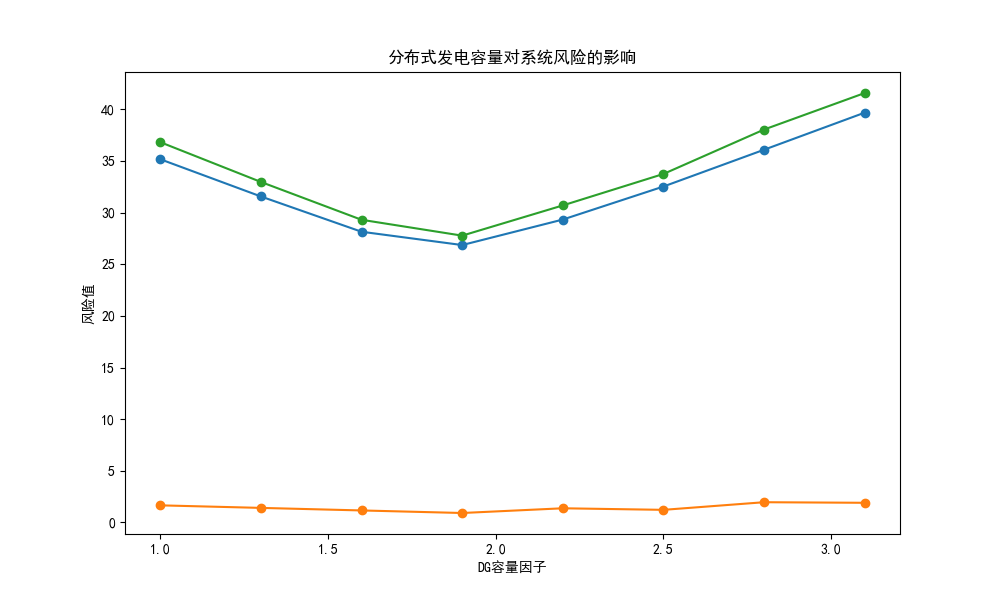
\includegraphics[width=0.8\textwidth]{problem2/dg_capacity_trending.png}
  \caption{分布式能源接入容量对系统风险的影响}
  \label{fig:risk_evolution}
\end{figure}

从图中可以看出,系统风险随着分布式能源接入容量的增加而呈现出先下降后上升的趋势。
在接入容量较小时,系统风险随着接入容量的增加而下降,说明分布式能源的接入能够有效降低系统风险。
然而,当接入容量达到一定程度后,系统风险又开始上升,这可能是由于 dg 节点本身的出力波动性和不确定性导致的。

同时,还有分馈线的风险占比随分布式能源接入容量变化的曲线图,如图 \ref{fig:line_risk_evolution} 所示。

\begin{figure}[htbp]
  \centering
  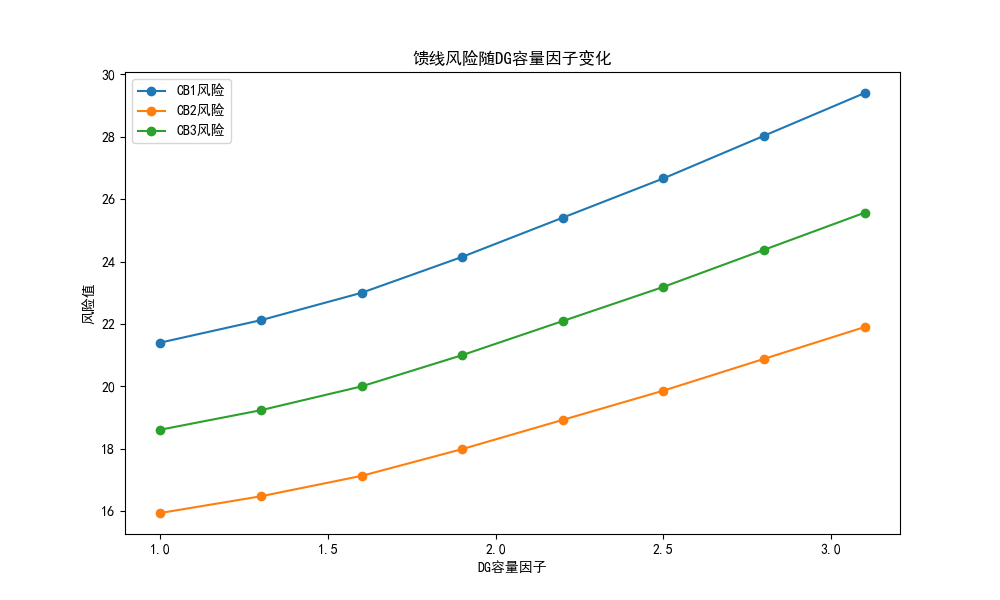
\includegraphics[width=0.8\textwidth]{problem2/dg_capacity_trending_feeder.png}
  \caption{馈线风险占比随分布式能源接入容量变化}
  \label{fig:line_risk_evolution}
\end{figure}

经过以上分析,可以得出:当容量因子为 1.9 时,系统的风险最低,降低到了约 27.77。

\section{模型分析检验}\label{sec:analysis_check}

\section{模型评价与推广}\label{sec:evaluation}

\section{附录}\label{sec:appendix}

\subsection{代码实现}\label{subsec:code}

% minted 环境构建速度较慢,因此暂时注释掉
% \inputminted{python}{Q1_risk_model.py}

\end{document}
